\documentclass[12pt,spanish]{article}
\usepackage[spanish]{babel}
\selectlanguage{spanish}
\usepackage[utf8]{inputenc}
\usepackage{color}
\usepackage{graphicx}
\usepackage{wrapfig}
\usepackage{float}
\usepackage[a4paper, total={6in, 8in}, margin=0.6in]{geometry}



\begin{document}

\begin{center}
    \fbox{\fbox{\parbox{5.5in}{\centering Responde las preguntas en el espacio provisto en la hoja de preguntas. si te quedas sin espacio para la respuesta, continúa del otro lado de la hoja.}}}

\vspace{0.2in}
\makebox[\textwidth]{Nombre y apellido:\enspace\hrulefill}

\vspace{0.2in}
\makebox[\textwidth]{Grupo:\enspace\hrulefill}

\vspace{0.2in}

    {\huge Examen de Informática}
\end{center}

\section{formato de texto}
    Escribe el siguiente texto y realiza los cambios de formato que se enumeran debajo.
    
    \begin{center}
      \centering
      La Mascota del mundial Rusia 2018
    \end{center}
   
    \begin{wrapfigure}{l}{0.35\textwidth}
        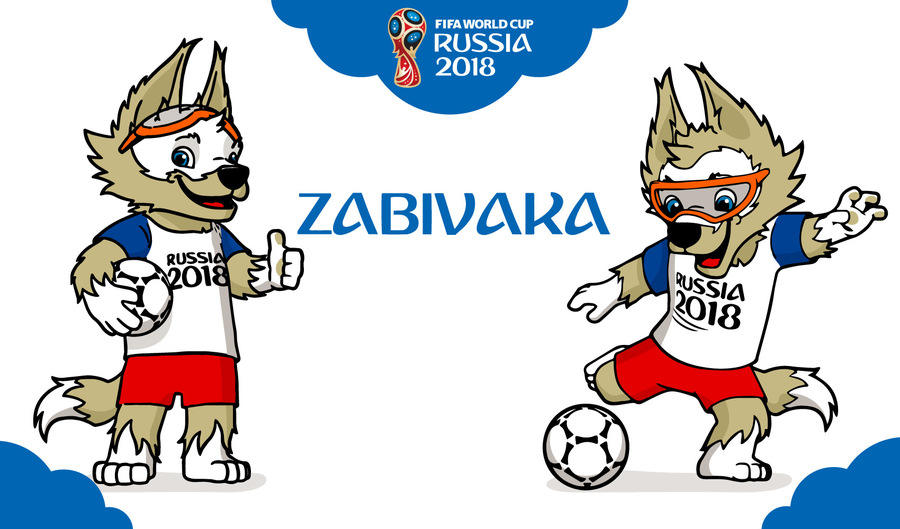
\includegraphics[width=0.35\textwidth]{rusia.jpg}
    \end{wrapfigure}

    La Copa Mundial de la FIFA Rusia 2018 está cada vez más cerca... ¡Solo faltan 14 días! Hasta que comience a rodar el balón, destacaremos diariamente un número relevante en la historia del torneo.
    
    La 14ª mascota oficial en la historia de la Copa Mundial de la FIFA es un lobo divertido, seductor y seguro de sí mismo que se llama Zabivaka.

  Zabivaka se ganó el cariño del mundo entero el año pasado durante la Copa FIFA Confederaciones, y ahora resulta imposible imaginar que Rusia 2018 se desarrolle sin este encantador lobo. El país anfitrión lo pudo conocer incluso antes, pues más de un millón de rusos votaron en FIFA.com para decidir la mascota oficial del Mundial que se celebrará en su territorio.
  
  La tradición de mascotas en la Copa Mundial de la FIFA se remonta al cachorro de león Willie en Inglaterra 1966. En cada una de las ediciones subsiguientes, el papel de la mascota se ha ido haciendo progresivamente más importante, y actualmente constituye un componente esencial del espectáculo.


  \vspace{0.1in}
  \underline{\textbf {Realiza los siguientes cambios al texto:}}
  \vspace{0.1in}
  
  \begin{enumerate}
    \item Inserta una imagen de la mascota del mundial en el lugar indicado
  \item Cambia el formato del título a fuente arial, 20pts, centrado, subrayado y de color azul
  \item Divide el tercer párrafo en 3 columnas
  \end{enumerate}

  \section{Teórico}
  \begin{enumerate}
    \item Describe la diferencia principal entre software y hardware 
  \item Haz una lista de al menos de 3 ejemplos de hardware y 3 de software 
  \item Explica con tus palabras qué es Internet 
  \end{enumerate}


\end{document}
